\documentclass{article}
\usepackage[top=1in,bottom=1in,left=1in,right=1in]{geometry}
\usepackage{listings}
\usepackage{hyperref}
\usepackage{color}
\usepackage[pdftex]{graphicx}
\usepackage{xspace}


\title{Models of FMDV in a Herd of Cattle}
\author{Drew Dolgert}
\date{\today}

\begin{document}
\maketitle
\abstract{There is significant data on the progress of FMDV within individual
cattle. This data describes both the progress of the disease and its variability
among individuals according to various effects. Obtaining multiple samples of
similar data for herds of infected cattle is impractical or inhumane, so
models extend understanding at an individual level to a herd level. This article
examines a family of models for FMDV progress within a herd in order to
understand how both the average progress of disease and an estimate of its
variability.}

\section{Introduction}
Focus on a putative herd of beef cattle of the same breed and similar life stage.
Build several models of varying complexity.

This will work with compartmental models in continuous time.
We will look at a series of models. A model is defined as a set
of states, transitions which modify the states, and rates for those
transitions. For each variant of a model, look at which of these
three is varied.


\section{FMDV progress within an individual}
\begin{figure}
\centerline{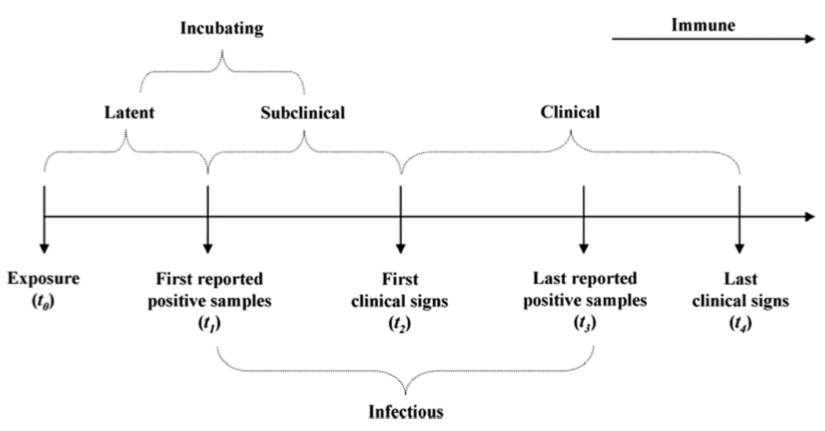
\includegraphics[width=9cm]{mardones_states}}
\caption{States of FMDV from Mardones et al.\cite{Mardones2010}.\label{fig:mardones_states}}
\end{figure}
\begin{figure}
\centerline{\begin{tabular}{llll}
\hline
FMD stage & time interval [days] & State Transition & Poisson & Distribution \\ \hline
Latent &  $t_1-t_0$ & $(I,0,0)$--$(I,1,0)$ & 3.59 & Weibull ($\alpha=1.782$, $\beta=3.974$) \\
Subclinical & $t_2-t_1$ & $(I,1,0)$--$(I,1,1)$ & 2.04 & Gamma ($\alpha=1.222$, $\beta=1.672$) \\
Incubation & $t_2-t_0$ & $(I,0,0)$--$(I,1,1)$ & 5.9 & Log logistic ($\gamma=0$, $\beta=5.3$, $\alpha=4.02$) \\
Infectious &  $t_3-t_1$ & $(I,1,0)$--$(R,0,1)$ & 4.39 & Gamma ($\alpha=3.969$, $\beta=1.107$) \\
Clinical Recovery & $t_4-t_2$ & $(I,1,1)$--$(R,0,0)$ & NA & NA
\end{tabular}}
\caption{From ``FMDV serotype O infection in domestic animals,''\label{fig:compartments}}
\end{figure}%
\begin{figure}
\centerline{\begin{tabular}{llll}
\hline
Viral Load & Infectiousness & Clinical Sign & Seen in FMDV \\ \hline
Susceptible & 0 & 0 & Susceptible state \\
Infected & 0 & 0 & Latent state \\
Infected & 0 & 1 & not seen \\
Infected & 1 & 0 & Infectious, sub-clinical \\
Infected & 1 & 1 & Infectious, clinical \\
Recovered & 1 & 1 & not seen \\
Recovered & 0 & 1 & Recovered, clinical \\
Recovered & 1 & 0 & not seen \\
Recovered & 0 & 0 & Recovered, sub-clinical
\end{tabular}}
\caption{This lists all possible states of an individual
with these three separate measurable traits. Listing all possible
states is a first step towards choosing how to represent
the states and transitions among those states.\label{fig:allstates}}
\end{figure}%
In an epidemiological context, a compartmental model reduces
the pathology of FMDV to whether inoculation and recovery have happened,
whether the animal is infectious, and whether the animal shows
visible clinical signs of infection. These differentiate among
viral load within the animal, shedding of virus, and visible
immune response. They create a table of possible states, shown
in Fig.~\ref{fig:allstates},
only some of which are witnessed for the progression of FMDV.

For continuous-time models, no two transitions are simultaneous,
so a chart of all possible transitions includes a transition
for a change in any one of the three traits. For instance,
there may be a transition from $(I,0,0)$, which represents
an infected state with no infectiousness or clinical sign,
to $(I,0,1)$ or to $(I,1,0)$ but no direct transition to $(I,1,1)$,
a state which is both infectious and clinical. The chart
of possible transitions is shown in Fig.~blah.
It is colored according to states described by Mardones
et al.\ in a review paper.

That paper focuses on those transitions most important for
the progress of disease, as defined from five observation
points, exposure at $t_0$, first reported positive sample
at $t_1$, first clinical sign at $t_2$, last reported positive sample at $t_3$,
and last clinical sign at $t_4$. A diagram of this timeline is
in Fig.~\ref{fig:compartments}.
The observations are implicitly ordered in time, as 0 through 4,
although this is not guaranteed for other diseases where, for instance,
clinical sign might precede infectiousness.
From these are defined five transitions, shown in Fig.~\ref{fig:compartments}.
The transition from clinical back to subclinical is excluded,
presumably because it is both less important and without
significant data. Note also that the end of infectiousness
coincides with the end of infection in this model, eliding
the two possible states, $(I,0,1)$ and $(R,0,1)$, in the
general model.

Mardones et al.\ offer two different ways to specify
when clinical signs begin. One is an Incubation transition. The
other is two transitions in a row, through the latent and subclinical
stages. These alternatives express conditional dependency.
If clinical signs depend upon infectiousness, then the two-step
process is appropriate. If they are independent, then the incubation
period is the correct representation. A simulation using
the incubation period would not guarantee that
infection occurs before incubation, except insofar as
the transition rates encourage this ordering.
A stochastic compartmental model represents independent
processes, such as becoming clinical and becoming
infectious, as transitions which affect different substates
of the system, so the alternative dependencies become
alternative representations of the compartmental model,
shown in Fig.~\ref{fig:individual_gspn}.
For neither representation do the allowed transitions correspond
exactly to those suggested by the time-ordered compartments
shown in Mardones et al., but they both capture
the most important stages of FMDV.

\begin{figure}
\centerline{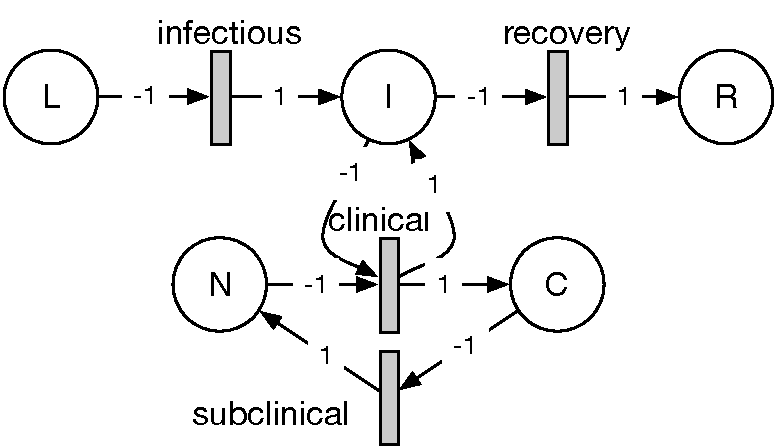
\includegraphics[width=9cm]{individual_gspn}}
\caption{The four compartmental states of an animal with FMDV
are represented by two categories, $(S,I,R)$ and $(N,C)$
where $N$ and $C$ represented not-clinical or clinical.
Computation proceeds by moving a token among $(S,I,R)$ and a
second token among $(N,C)$. Rectangles represent transitions,
which are enabled only when tokens are at all input edges to the
transition.\label{fig:individual_gspn}}
\end{figure}%

Simulations of both models show that, while average rates
are the same, the distribution
of times to infection or recovery can be quite different.
How much this matters depends on the application, which
here is prediction of prevalence within a herd.

\section{Herd Models}
Spread of infection within a herd of cattle is complicated.
Using a compartmental model built from the individual
models above distills complication into variation in
individual compartments and transitions, contact structure,
and infection rate given that contact structure.
How cattle fraternize in a field can be seen as a
time-dependent contact graph whose structure is 
distinct from the infection process which takes place
on that graph. For instance, if the shortest path between
two individuals in the graph is four individuals long, then
\emph{any\/} disease will require two latent periods
to travel from one individual to another.

\begin{itemize}
  \item Exponential or non-exponential individual model.
  \item Time-dependent contact hazard or frequency-dependent contact.
\end{itemize}

\bibliography{cattleherd}
\bibliographystyle{plain}
\end{document}
